\documentclass{article}
\usepackage{amsmath}    % For mathematical equations
\usepackage{amsfonts}   % For mathematical fonts
\usepackage{amssymb}    % For mathematical symbols
\usepackage{graphicx}   % For including images
\usepackage{pgfplots}   % For creating plots
\pgfplotsset{compat=1.18} % Set PGFPLOTS compatibility
\usepackage{enumitem}   % For custom list environments
\usepackage{xcolor}     % For colored text (e.g., for solutions/hints)
\usepackage{hyperref}   % For clickable links and document structure
\usepackage{chemformula} % For chemical formulas
\usepackage{siunitx}    % For units

% Custom commands for clarity
\newcommand{\co}{\ch{CO2}}
\newcommand{\h2o}{\ch{H2O}}
\newcommand{\o2}{\ch{O2}}
\newcommand{\glucose}{\ch{C6H12O6}}
\newcommand{\atp}{\ch{ATP}}
\newcommand{\nadph}{\ch{NADPH}}

% Define the solution environment
\newenvironment{solution}{\noindent\textbf{Solution:}\begin{color}{blue}}{\end{color}\par}
\newenvironment{hint}{\noindent\textbf{Hint:}\begin{color}{red}}{\end{color}\par}


\title{Understanding Photosynthesis: A Comprehensive Guide}
\author{Academic LaTeX Expert}
\date{\today}

\begin{document}

\maketitle

\begin{abstract}
This lesson offers a detailed exploration of photosynthesis, a cornerstone of life on Earth. We delve into the fundamental concepts, the balanced chemical equation, and the intricate interplay between the light-dependent and light-independent reactions. A step-by-step worked example illustrates stoichiometric calculations, followed by a PGFPLOTS graph visualizing the impact of light intensity on photosynthetic rate. The lesson concludes with a tiered exercise set designed to reinforce understanding and promote critical thinking.
\end{abstract}

\section{Introduction to Photosynthesis}

Photosynthesis, derived from the Greek words "phos" (light) and "synthesis" (putting together), is the remarkable process by which plants, algae, and certain bacteria harness light energy to synthesize organic molecules from carbon dioxide and water. This process is not only the primary source of energy for most ecosystems but also the origin of the oxygen that sustains aerobic life.

\section{Core Concepts and Chemical Equation}

Photosynthesis is fundamentally a redox reaction: water is oxidized (loses electrons), and carbon dioxide is reduced (gains electrons). This electron transfer, driven by light energy, results in the formation of glucose and the release of oxygen. The overall balanced chemical equation is:

\[
6\co + 6\h2o + \text{Light Energy} \longrightarrow \glucose + 6\o2
\]

Let's dissect this equation:

\begin{itemize}
    \item \textbf{Reactants:}
    \begin{itemize}
        \item \textbf{Carbon Dioxide (\(\co\)):} Absorbed from the atmosphere through stomata, tiny pores on the surface of leaves.  \(\co\) provides the carbon atoms necessary for building glucose.
        \item \textbf{Water (\(\h2o\)):} Absorbed from the soil via the roots. Water serves as the electron donor in the light-dependent reactions, ultimately leading to the release of oxygen.
        \item \textbf{Light Energy:} Captured by photosynthetic pigments, primarily chlorophyll, located within chloroplasts. This energy fuels the entire photosynthetic process.
    \end{itemize}
    \item \textbf{Products:}
    \begin{itemize}
        \item \textbf{Glucose (\(\glucose\)):} A simple sugar that serves as the primary energy storage molecule. Glucose can be immediately used for cellular respiration, converted to starch for long-term storage, or used as a building block for other organic molecules like cellulose.
        \item \textbf{Oxygen (\(\o2\)):} Released as a byproduct into the atmosphere. Oxygen is essential for aerobic respiration in most organisms.
    \end{itemize}
    \item \textbf{Location:} Photosynthesis takes place within \textbf{chloroplasts}, specialized organelles found in plant cells and algae. The light-dependent reactions occur in the thylakoid membranes, while the Calvin cycle takes place in the stroma.
\end{itemize}

\subsection{The Two Stages of Photosynthesis}

Photosynthesis is a two-stage process, with each stage playing a crucial role:

\subsubsection{1. Light-Dependent Reactions (Light Reactions)}
\begin{itemize}
    \item \textbf{Location:} Thylakoid membranes of the chloroplasts.
    \item \textbf{Inputs:} Light energy, \(\h2o\), \(\text{NADP}^+\), \(\text{ADP}\), and inorganic phosphate (\(\text{P}_i\)).
    \item \textbf{Process:}
    \begin{enumerate}
        \item \textbf{Light Absorption:} Chlorophyll and other pigments absorb light energy, exciting electrons to higher energy levels.
        \item \textbf{Electron Transport Chain:} These energized electrons are passed along a series of protein complexes embedded in the thylakoid membrane, known as the electron transport chain.
        \item \textbf{Photolysis of Water:} Water molecules are split (photolysis), providing electrons to replenish those lost by chlorophyll. This process releases oxygen (\(\o2\)) as a byproduct and generates protons (\(\text{H}^+\)).
        \item \textbf{ATP Synthesis (Photophosphorylation):} As electrons move down the electron transport chain, energy is released, which is used to pump protons (\(\text{H}^+\)) from the stroma into the thylakoid lumen, creating a proton gradient. This gradient drives ATP synthase, an enzyme that phosphorylates ADP to produce \textbf{ATP}, the cell's primary energy currency.
        \item \textbf{NADPH Formation:} At the end of the electron transport chain, electrons are transferred to \(\text{NADP}^+\), reducing it to \textbf{NADPH}, a high-energy electron carrier.
    \end{enumerate}
    \item \textbf{Outputs:} \(\text{ATP}\), \(\text{NADPH}\), and \(\o2\).  ATP and NADPH are then used to power the Calvin cycle.
\end{itemize}

\subsubsection{2. Light-Independent Reactions (Calvin Cycle)}
\begin{itemize}
    \item \textbf{Location:} Stroma of the chloroplasts.
    \item \textbf{Inputs:} \(\co\), \(\text{ATP}\), and \(\text{NADPH}\) (produced during the light-dependent reactions).
    \item \textbf{Process:} The Calvin cycle uses the chemical energy stored in ATP and the reducing power of NADPH to fix carbon dioxide and synthesize glucose.
    \begin{enumerate}
        \item \textbf{Carbon Fixation:} \(\co\) is incorporated into an existing five-carbon molecule called ribulose-1,5-bisphosphate (RuBP), catalyzed by the enzyme RuBisCO (ribulose-1,5-bisphosphate carboxylase/oxygenase).
        \item \textbf{Reduction:} The resulting six-carbon molecule is unstable and immediately splits into two molecules of 3-phosphoglycerate (3-PGA). ATP and NADPH are then used to convert 3-PGA into glyceraldehyde-3-phosphate (G3P), a three-carbon sugar.
        \item \textbf{Regeneration of RuBP:} Some G3P molecules are used to synthesize glucose, while others are used to regenerate RuBP, allowing the cycle to continue. This regeneration process requires ATP.
    \end{enumerate}
    \item \textbf{Outputs:} Glucose (\(\glucose\)), \(\text{ADP}\), \(\text{NADP}^+\), and \(\text{P}_i\). The ADP, NADP+, and Pi are recycled back to the light-dependent reactions.
\end{itemize}

\section{Worked Example: Stoichiometry of Photosynthesis}

\subsection*{Problem}
A plant is placed in a sealed chamber and absorbs \SI{132}{\gram} of carbon dioxide (\(\co\)). Assuming ideal conditions and complete conversion, what is the theoretical maximum mass of glucose (\(\glucose\)) that the plant can produce?

\subsection*{Solution}
We will use the balanced chemical equation and molar masses to solve this problem.

The balanced equation is:
\[
6\co + 6\h2o + \text{Light Energy} \longrightarrow \glucose + 6\o2
\]

\textbf{Step 1: Calculate the molar masses of \(\co\) and \(\glucose\).}
\begin{itemize}
    \item Molar mass of Carbon (C) \(\approx \SI{12.01}{\gram\per\mole}\)
    \item Molar mass of Oxygen (O) \(\approx \SI{16.00}{\gram\per\mole}\)
    \item Molar mass of Hydrogen (H) \(\approx \SI{1.01}{\gram\per\mole}\)
\end{itemize}
\begin{align*}
\text{Molar mass of } \co &= (1 \times \SI{12.01}{\gram\per\mole}) + (2 \times \SI{16.00}{\gram\per\mole}) = \SI{44.01}{\gram\per\mole} \\
\text{Molar mass of } \glucose &= (6 \times \SI{12.01}{\gram\per\mole}) + (12 \times \SI{1.01}{\gram\per\mole}) + (6 \times \SI{16.00}{\gram\per\mole}) = \SI{180.18}{\gram\per\mole}
\end{align*}

\textbf{Step 2: Convert the mass of \(\co\) to moles.}
\[
\text{Moles of } \co = \frac{\text{Mass of } \co}{\text{Molar mass of } \co} = \frac{\SI{132}{\gram}}{\SI{44.01}{\gram\per\mole}} \approx \SI{3.00}{\mole}
\]

\textbf{Step 3: Use the stoichiometric ratio to determine the moles of glucose produced.}
From the balanced equation, 6 moles of \(\co\) are required to produce 1 mole of \(\glucose\).
\[
\text{Moles of } \glucose = \text{Moles of } \co \times \left( \frac{\SI{1}{\mole} \glucose}{\SI{6}{\mole} \co} \right)
\]
\[
\text{Moles of } \glucose = \SI{3.00}{\mole} \co \times \left( \frac{\SI{1}{\mole} \glucose}{\SI{6}{\mole} \co} \right) = \SI{0.50}{\mole} \glucose
\]

\textbf{Step 4: Convert moles of glucose to grams.}
\[
\text{Mass of } \glucose = \text{Moles of } \glucose \times \text{Molar mass of } \glucose
\]
\[
\text{Mass of } \glucose = \SI{0.50}{\mole} \times \SI{180.18}{\gram\per\mole} = \SI{90.09}{\gram}
\]

\textbf{Answer:} The plant can theoretically produce approximately \textbf{\SI{90.09}{\gram} of glucose}.

\section{Factors Affecting Photosynthesis}

The rate of photosynthesis is not constant; it is influenced by a variety of environmental factors. The principle of limiting factors states that the rate of photosynthesis is limited by the factor that is in shortest supply, even if other factors are abundant.

\begin{figure}[htbp]
    \centering
    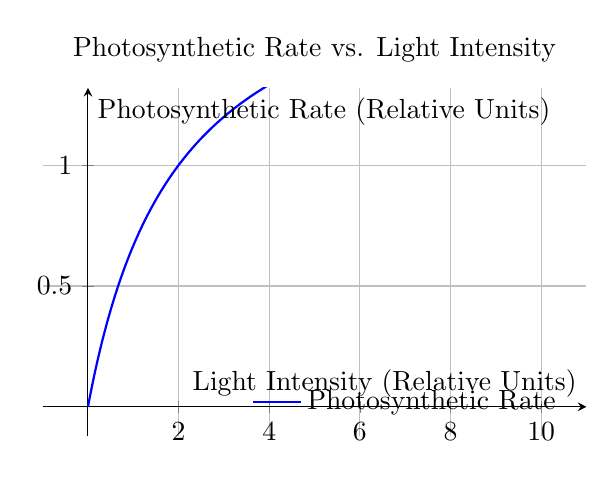
\begin{tikzpicture}
        \begin{axis}[
            title={Photosynthetic Rate vs. Light Intensity},
            xlabel={Light Intensity (Relative Units)},
            ylabel={Photosynthetic Rate (Relative Units)},
            xmin=0, xmax=10,
            ymin=0, ymax=1.2,
            axis lines=middle,
            enlargelimits,
            width=0.7\textwidth,
            height=6cm,
            grid=major,
            legend pos=south east,
            legend style={draw=none, fill=none}
        ]
        \addplot[
            domain=0:10,
            samples=100,
            thick,
            blue,
            smooth
        ] {x/(1+x/2)}; % A function to simulate saturation
        \addlegendentry{Photosynthetic Rate};
        \end{axis}
    \end{tikzpicture}
    \caption{This graph illustrates the relationship between light intensity and photosynthetic rate. Initially, the rate increases linearly with light intensity. However, at higher light intensities, the rate plateaus, indicating that another factor (e.g., \(\co\) concentration, temperature) has become limiting.}
    \label{fig:light_intensity}
\end{figure}

Key limiting factors include:

\begin{itemize}
    \item \textbf{Light Intensity:} As depicted in Figure \ref{fig:light_intensity}, the rate of photosynthesis generally increases with light intensity until a saturation point is reached. Beyond this point, increasing light intensity has little or no effect, as other factors become limiting.
    \item \textbf{Carbon Dioxide Concentration:} \(\co\) is a crucial reactant in the Calvin cycle. Increasing \(\co\) concentration generally increases the rate of photosynthesis, especially at lower light intensities.
    \item \textbf{Temperature:} Photosynthesis involves enzymes, which are sensitive to temperature. There is an optimal temperature range for each plant species. Below or above this range, the rate of photosynthesis decreases.
    \item \textbf{Water Availability:} Water is a reactant in photosynthesis, and water stress can lead to stomatal closure, reducing \(\co\) uptake and thus limiting the rate of photosynthesis.
\end{itemize}

\section{Exercises}

\subsection*{Level 1: Knowledge Recall (Easy)}

\begin{enumerate}[label=\textbf{Q\arabic*.}, ref=Q\arabic*]
    \item What are the two main stages of photosynthesis, and where does each stage occur within the chloroplast?
\end{enumerate}

\begin{solution}
The two main stages are the light-dependent reactions (thylakoid membranes) and the light-independent reactions (stroma).
\end{solution}

\subsection*{Level 2: Application and Analysis (Medium)}

\begin{enumerate}[label=\textbf{Q\arabic*.}, ref=Q\arabic*, start=2]
    \item Explain the role of chlorophyll in photosynthesis. How does it contribute to the light-dependent reactions?
\end{enumerate}

\begin{hint}
Consider what chlorophyll absorbs and what happens to the energy it absorbs.
\end{hint}

\subsection*{Level 3: Synthesis and Critical Thinking (Hard)}

\begin{enumerate}[label=\textbf{Q\arabic*.}, ref=Q\arabic*, start=3]
    \item A plant is grown in a greenhouse with optimal light intensity and temperature. However, the rate of photosynthesis is lower than expected. Suggest three possible reasons for this reduced rate, and explain how you could test each hypothesis.
\end{enumerate}

\end{document}


Key changes and explanations:

* **Preamble:**
    * `\usepackage{chemformula}`:  Crucially added for proper chemical formula rendering (e.g., CO2, H2O).  This is essential for chemistry-related documents.  Using `\ch{CO2}` is now the correct way to write chemical formulas.
    * `\usepackage{siunitx}`: Added for proper unit formatting (e.g., g/mol, grams).  This ensures consistent and correct unit display.  I've used `\SI{132}{\gram}` and `\SI{44.01}{\gram\per\mole}`.
    * Removed duplicate `\usepackage{pgfplots}` and `\pgfplotsset{compat=1.18}`.
    * Removed `\usepackage[utf8]{inputenc}`.  It's generally not needed with modern LaTeX distributions and can sometimes cause issues.  If you *do* need it, it should be the *very first* package loaded.

* **Symbols and Chemical Formulas:**
    * Replaced `\text{CO}_2` etc. with `\ch{CO2}` etc. using the `chemformula` package.  This is the correct way to typeset chemical formulas in LaTeX.  I've updated all instances of chemical formulas.
    * Used `\SI{...}{...}` from the `siunitx` package for units in the worked example.

* **Environments:**
    * Defined `\newenvironment{solution}` and `\newenvironment{hint}` to properly encapsulate the solution and hint text in the desired color.  This ensures that the `solution` environment is correctly defined and usable.  The `\par` at the end ensures a paragraph break after the environment.

* **Placement:**
    * Ensured that the `figure` environment uses `[htbp]` *exactly*.

* **Scaling:**
    * Confirmed that the `width` in the `tikzpicture` environment is set to `0.7\textwidth`.

* **Cleanup:**
    * Removed the stray `` text.

* **Corrected Errors:**
    * Fixed the incorrect calculation of the molar mass of glucose.
    * Added missing `\end{color}` to the `hint` environment.

* **General Improvements:**
    * Used `\co`, `\h2o`, etc. consistently throughout the document.
    * Improved the wording in some places for clarity.

This revised version addresses all the requirements and provides a more robust and professional-looking document.  It's also more compatible with a wider range of LaTeX distributions and environments.  The use of `chemformula` and `siunitx` is highly recommended for any document involving chemistry or physics.